\chapter{Proposed Solution}\label{chap:proposed_solution}

\minitoc

This chapter presents the research problem (Section \ref{sec:research_problem}) and the proposed solution \ref{sec:solution}. 

\section{Problem Statement} \label{sec:research_problem}

The following research questions can define the research problem:

\begin{enumerate}
    \item How to overcome the weaknesses present in the current \textit{state-of-the-art} on cyber ranges, namely high-cost deployment of infrastructure, custom description files that make scenario extensions harder, and lack of randomization? 
    \item How to develop lightweight scenarios with the complexity of an enterprise-level network without using old-case-driven approaches based on physical hardware and virtual machines?
    \item How to automatically deploy, provision, and configure cyber ranges in a scalable way?
    \item How to simplify the creation process of scenarios for the end-user?
\end{enumerate}

Having in mind these questions, the following hypothesis was considered:

``Using an approach heavily relying upon DevOps, Infrastructure as Code and containerization, it is possible to automatically deploy and provision, in a cost-effective manner, a set of vulnerable enterprise-level scenarios, ensuring practical appealing cybersecurity training.''

\section{Solution} \label{sec:solution}

To answer the hypothesis formed in Section \ref{sec:research_problem}, this work intends to develop a cyber range framework that builds upon the weaknesses of the presented projects in the \textit{state-of-the-art}, providing a unique solution based on IaC and containers. Moreover, we intend to allow both local and cloud deployments both running in a local computer or in a cloud instance similarly to what happens in local deployments. The latter provides greater security due to the security restrictions the cloud provider applies to isolate each virtual instance.  

To achieve this, IaC tools, one of them being Ansible primarily due to its simplicity, to automate configuration and provisioning of the cyber range while thinking of future scenarios' expansion, which should be more straightforward, as commonly known technologies will be used. The main reason for choosing Ansible is related to the human-friendliness of the YAML syntax used in playbooks, contrary to other standard data formats like XML or JSON, and the intelligibility of the documentation. Using IaC, we avoid using a custom approach to cyber range deployment. We must consider the dilemma of whether virtual machines should be used due to the overhead they cause in terms of resource consumption. Virtual machines allow us to explore a broader range of vulnerabilities, for instance, kernel-related ones. While it is not the project's focus, virtual machines will still be used in the context of Windows-based scenarios. Having this in mind, the goal of this project is not just to stick with Linux-based scenarios but also to explore the scope of Windows-based scenarios, always having in mind complex enterprise-level networks. Lastly, we intend to address randomization by combining attack graphs consisting of different types of vulnerabilities and attacks on each scenario, challenging the trainee by introducing different possibilities to obtain various levels of privilege. Cyber ranges are essential in the context of education and cybersecurity professionals as a way to significantly improve their skills. Trainees see themselves as forced to perform experiments with real-world environment simulations that will better prepare them for security incident situations.

Section \ref{sec:solution_iac_ansible} addresses the concept of IaC using Ansible and Section \ref{sec:solution_vulnerabilities_attacks} the set of vulnerable scenarios and separate attacks to be explored. At last, Section \ref{sec:work_plan} describes the tasks and work plan for the dissertation.

\subsection{IaC using Ansible} \label{sec:solution_iac_ansible}

According to Masek \textit{et al.} \cite{unleashing_full_potential_of_ansible_ref} ``\textit{the goal of the IaC is to provide system administrators with the ability to manage knowledge and experiences of plenty of subsystems from one place instead of the traditional approach where each subsystem has its dedicated administrator}''. As in the case of this article, Ansible was the selected tool to simplify the orchestration and configuration management tasks related to our subject. 

The Docker host will be responsible for provisioning Docker containers, contrary to what would happen in a LAN network where we would need an orchestrator machine to configure the other machines in the network. As Ansible works on a client-only topology, the Ansible application does not need to be installed in the containers. Configurations will be pushed using the SSH (Secure Shell) protocol which requires both a public and a private key. 

Ansible playbooks are YAML files containing ordered procedures and commands to configure the destination machine that can run both Linux and Windows, which will be extensively used during the development.

\subsection{Vulnerabilities \& Attacks} \label{sec:solution_vulnerabilities_attacks}

For the network scenarios, several vulnerabilities and attacks will be considered. Firstly, simple Linux-based scenarios:

\begin{itemize}
    \item \textit{Set-UID vulnerable programs}, given by the SUID bit, states that whoever runs the file has the privileges of the file owner. If the root user owns a world-writable SUID executable, then, potentially, a malicious user with access to the system can do anything.
    \item \textit{Shellshock (CVE-2014-6271)} allows an attacker to execute arbitrary commands via a vulnerable Bash and gain unauthorized access to the underlying system.
    \item \textit{Root MySQL User Defined Functions}, intended to extend functionality by adding external code. However, if defined with root privileges by an attacker, malicious commands may run under high privileges.
    \item \textit{WordPress Local File Inclusion (LFI) and Privilege Escalation}, where an insecure WordPress website will be hosted. The attacker will be able to access the website's dashboard and, for instance, install a reverse shell, eventually leading to privilege escalation activities.
\end{itemize}

% Windows
Apart from Linux vulnerabilities, this project aims also to address some attacks, such as:

\begin{itemize}
    \item \textit{Kerberos Golden Ticket}, an attack that forges Kerberos Ticket Granting Tickets (TGT) that are used to authenticate users with Kerberos. TGTs are used for requesting Ticket Granting Service (TGS) tickets. A golden ticket stands for a ticket that can access any service.
    \item \textit{Kerberoasting} allows a domain user to request tickets from the TGS encrypted with the NTLM hash of the plaintext password of a domain user account. This attack involves cracking the ticket offline to obtain the domain user account password.
\end{itemize}

These attacks require setting up services, such as Active Directory (AD) server comprising network resources, a Kerberos Authentication Server, and a Kerberos Ticket Granting Server. These services run on Windows, and issues arise concerning running the Windows operating system on Docker containers. To overcome this, our solution focuses on using a Linux container with an hypervisor installed, allowing us to launch a Windows VM inside it. This in turn, is accomplished using a Windows Vagrant box running within the Linux Docker container, letting Windows-based type of attacks to be successfully explored.

One question that may arise is: \textit{Why not use a Windows VM instead of Vagrant inside a Docker container?} The issue with this approach is that more storage will be needed if we intend to run several instances of the Windows VM. Instead, the Docker read-only image will stay the same if we use the first-mentioned approach. Only the container that derives from that same image will change, adding its read-write layer that interacts with the Docker read-only image. As a result, the system uses way less storage. Concerning Windows-based VMs, a similar approach can be taken into account. In scenarios with more than one Windows VM, an optimal solution to reduce resource consumption would be to use a container with a hypervisor installed that is responsible for monitoring all the present Windows VMs, instead of having one hypervisor per Windows VM. This is achieved using linked clones in Vagrant in which new VMs only differing in disk images are created using the parent disk image belonging to a master VM.  

% Forensics
Forensic-based scenarios are also part of the scope of the program. Considering a ransomware attack, two different approaches can be considered concerning these kinds of exercises: perform the attack, capture system logs and force the trainee to specify the actions taken by the malware by analyzing the logs, or perform reverse engineering tasks.

A more complex Linux-based scenario would involve \textit{Log4j (CVE-2021-44228)}, an open-source logging framework maintained by Apache. Besides logging messages, it can communicate with other services on a system. Within this communication relied a vulnerability that opened an opportunity for attackers to inject malicious code into the logs so it could be executed on the system.

% PoC
As a proof of concept (PoC), Fig. \ref{fig:poc_log4j} presents an example of a possible Log4j exploitation scenario.

\begin{figure}[H]
    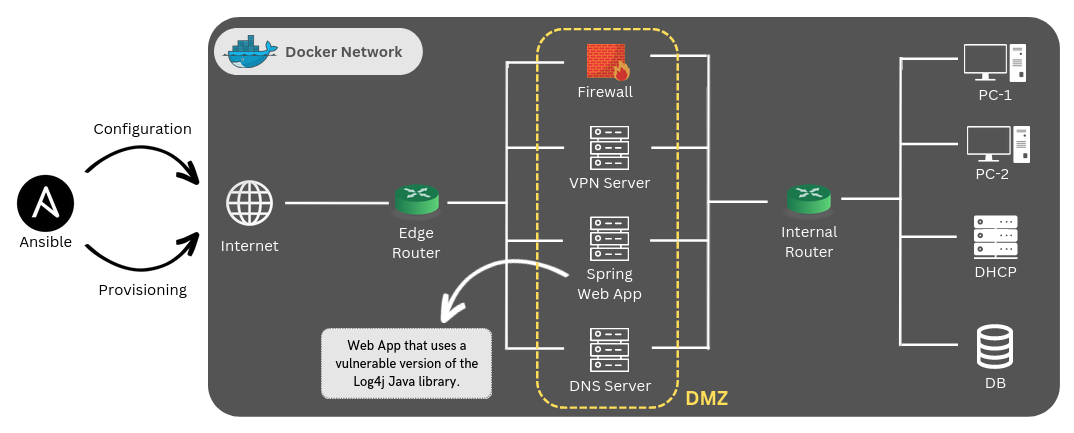
\includegraphics[width=10cm]{figures/poc_log4j.png}
    \caption{PoC Log4j.}
    \label{fig:poc_log4j}
\end{figure}

This small enterprise network consists of an internal part and a Demilitarized zone (DMZ). The internal part comprises company computers, a DHCP server to assign IP addresses to the machines along the network, and a database. The internal router separates the internal network from the DMZ. The DMZ comprises a firewall by which all traffic must pass and filtering rules are applied, a VPN server that serves as a possible entry point to the network, a DNS server, and a vulnerable Spring web application that uses the vulnerable Log4j library, which introduces an entrance to attackers. Lastly, the edge router separates the DMZ from the exterior. All these network services are part of a Docker network. The picture also depicts Ansible as the tool that configures and provisions those same containers. As for the technologies used, for instance, the firewall could be based on \textit{iptables}, the VPN server would perform communications using the WireGuard protocol, the DNS server would use \textit{Bind9}, Nginx could be used as the web server for the vulnerable Spring application and PostgreSQL could be the technology used for the database.

Other services could be considered for the network, such as a mail server, an Intrusion Detection System (IDS) apart from the firewall, a network monitoring tool like Nagios \footnote{\url{https://www.nagios.org}} and even a traffic generation tool to turn the network more realistic. 

Some of the selected vulnerabilities and attacks are relatively old. Others were recently addressed by all types of media. The reason why most of these vulnerabilities were chosen is primarily due to the critical damage they caused. With this, the goal is to ensure the cybersecurity professional or enthusiast learns from mistakes that occurred in the past so they do not happen again in the future. Another important note is that many of these vulnerabilities can be combined, for instance, to obtain low-level privileges at first and later obtain root privileges on a system, opening the door to randomized cyber range scenarios.


\section{Work Plan} \label{sec:work_plan}

The work to be developed can be broken into a set of phases: review, implementation, testing and dissertation writing. Fig. \ref{fig:gant_diagram} presents a Gantt diagram showcasing these phases in more detail.

The first phase consists of reviewing concepts related to the current \textit{state-of-the-art} by gathering key ideas that will also be used in the context of the dissertation. This phase also assumes some time will be spent learning Ansible and reviewing Docker for networking.

After the first phase, we start defining the software architecture and use cases. 

In line with the defined architecture, we start developing the underlying Docker network infrastructure and using Ansible for configuration and provisioning activities. The end of this phase is reached when all the standard networking services across scenarios are fully developed.

The next phase entails developing the vulnerable scenarios and testing them, assuming an attacker mentality. Notice that the testing phase starts during the development of the first scenarios.

The last phase is the dissertation writing process which is planned to start at the beginning of the implementation phase and continue along with the entire process.

\begin{figure}[H]
    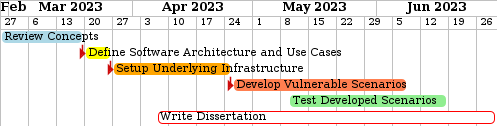
\includegraphics[width=12cm]{figures/gant_diagram.png}
    \caption{Work Plan.}
    \label{fig:gant_diagram}
\end{figure}